\documentclass{beamer}
\usepackage[utf8]{inputenc}
\usepackage{graphicx}
\author[Sowmya Vajjala]{Instructor: Sowmya Vajjala}

\title[LING 410X]{LING 410X: Language as Data}
\subtitle{Semester: Spring '18}

\date{5 Apr 2018}

\institute{Iowa State University, USA}
%%%%%%%%%%%%%%%%%%%%%%%%%%%

\begin{document}

\begin{frame}\titlepage
\end{frame}

\begin{frame}
\frametitle{Class Outline}
\begin{itemize}
\item Update on Assignment 5/mallet/topicmodels
\item Introduction to Stylo R package
\item Exercise with Stylo
\item Reminder: Assignment 5 - submit this weekend.
\item Reminder: Project initial report - submit this weekend.
\end{itemize}
\end{frame}

\begin{frame}
\frametitle{topic models}
\begin{itemize}
\item IT support did not manage to make mallet work on lab computers!
\item So, work with topic models, reduce those numbers in my tutorial (iter=50, thin=25 - this will perhaps work) 
\item If you complete this, move on to the next slides. 
\end{itemize}
\end{frame}

\begin{frame}
\frametitle{}
For those who already finished Assignment 5: 
Work with Stylo package in R by reading the documentation/based on the papers you read on Tuesday\\
\footnotesize \url{https://sites.google.com/site/computationalstylistics/stylo}
\end{frame}

\begin{frame}
\frametitle{Working with stylo}
\begin{itemize}
\item Installation instructions: \\ \url{https://sites.google.com/site/computationalstylistics/stylo}
\item Corpus to work with: There is a zip file on Canvas, stylocorpus.zip. 
\item Task: Learning to cluster texts together
\item Requirement: In the working directory where you call stylo() function in the stylo library, it expects to see a folder called corpus (lowercase) containing the text files you want to cluster
\item Useful links:
\\ \url{https://cran.r-project.org/web/packages/stylo/stylo.pdf}
\\ stylo\_howto.pdf on Canvas.
\end{itemize}
\end{frame}

\begin{frame}
\frametitle{Things to think about}
\begin{itemize}
\item How do the cluster arrangements change when you change: words to ngrams of different sizes? when you change other settings (MFW)? What are those other settings?
\item What is the best way of doing cluster visualizations in Stylo? (If you read those two articles from Tuesday, you will know)
\item Post your observations in the forum for today's date.
\end{itemize}
\end{frame}

\begin{frame}
\frametitle{Next week}
\begin{itemize}
\item Discussion of your observations from working with stylo
\item Discussion on what calculations stylo performs to get those visuals
\item Clustering - quick overview (using stylo)
\end{itemize}
\end{frame}

\end{document}

\begin{frame}
\frametitle{Stylo - doing cluster analysis}
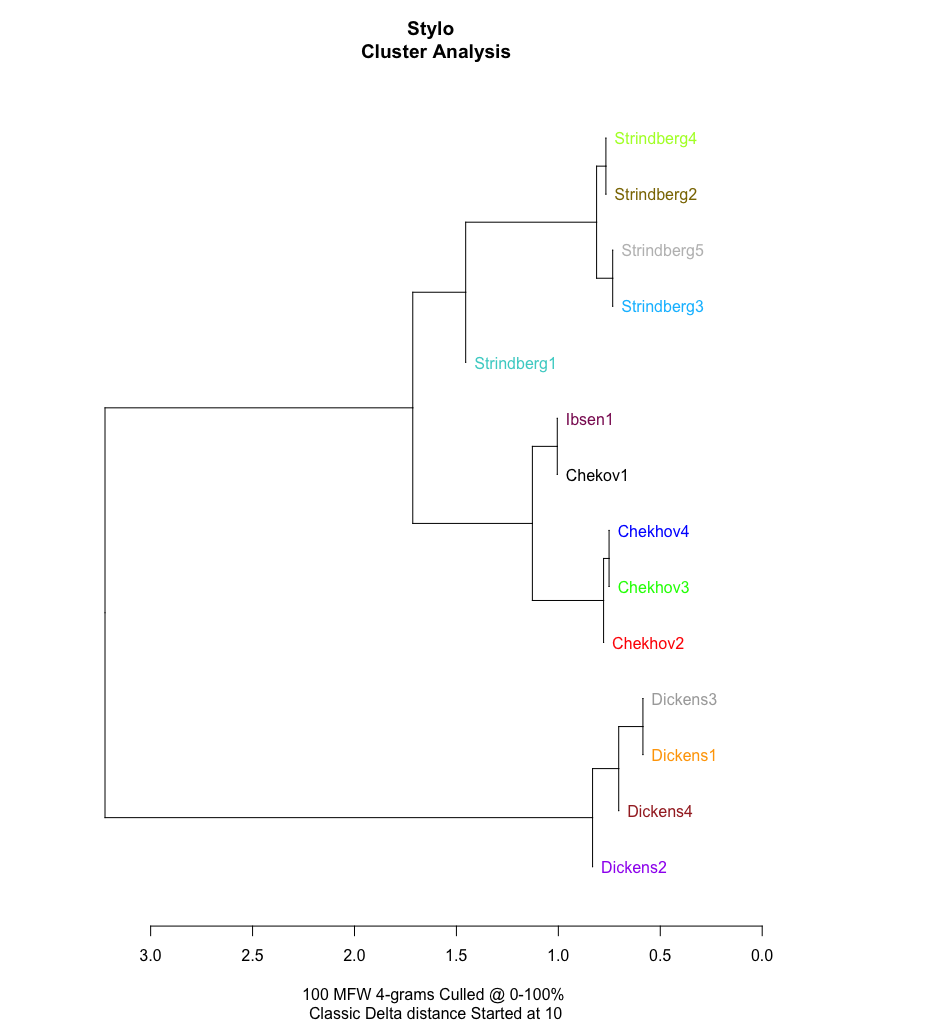
\includegraphics[width=0.78\textwidth]{ClusteringExample.png}
\end{frame}

\begin{frame}
\frametitle{Rolling Delta - knowing the author of an unknown text}
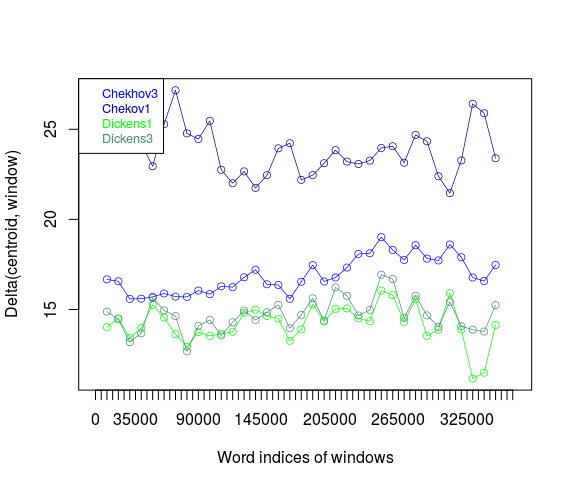
\includegraphics[width=0.8\textwidth]{RollingDeltaExample.png}
\end{frame}


%Discuss with diff plots changing settings on Tuesday.
